\section{Resultados}

A Tabela~\ref{tab:cv-modelos} resume o desempenho médio nos cinco folds
agrupados por imagem. A ConvNeXt-Tiny, modelo central deste estudo, obteve AUC
ROC de $0{,}9709\pm0{,}0059$ e AUC PR de $0{,}9607\pm0{,}0121$. Esses valores
indicam alta capacidade de ranquear células normais e anormais antes da escolha
de um limiar operacional. A comparação complementar com ResNet-50 ficou muito
próxima, com AUC ROC de $0{,}9668\pm0{,}0082$ e AUC PR de
$0{,}9513\pm0{,}0186$.

\begin{table}[H]
\centering
\caption{Desempenho da ConvNeXt-Tiny e comparação complementar com ResNet-50
por validação cruzada agrupada. Valores em média $\pm$ desvio-padrão, limiar
0,50 e sem TTA.}
\label{tab:cv-modelos}
\kariellycompacttablefont
\kariellytablecols
\begin{tabular}{lcc}
\toprule
Métrica & ConvNeXt-Tiny & ResNet-50 \\
\midrule
AUC ROC & $0{,}9709\pm0{,}0059$ & $0{,}9668\pm0{,}0082$ \\
AUC PR & $0{,}9607\pm0{,}0121$ & $0{,}9513\pm0{,}0186$ \\
Acurácia balanceada & $0{,}9091\pm0{,}0115$ & $0{,}9105\pm0{,}0139$ \\
Sensibilidade & $0{,}8994\pm0{,}0480$ & $0{,}9001\pm0{,}0344$ \\
Especificidade & $0{,}9188\pm0{,}0400$ & $0{,}9210\pm0{,}0264$ \\
\emph{F1} & $0{,}8926\pm0{,}0128$ & $0{,}8943\pm0{,}0161$ \\
MCC & $0{,}8189\pm0{,}0208$ & $0{,}8205\pm0{,}0262$ \\
Kappa & $0{,}8164\pm0{,}0223$ & $0{,}8195\pm0{,}0271$ \\
\emph{Brier score} & $0{,}0699\pm0{,}0079$ & $0{,}0671\pm0{,}0096$ \\
\bottomrule
\end{tabular}
\end{table}

Nas métricas calculadas no limiar 0,50, os modelos apresentaram comportamento
operacional praticamente equivalente. A ResNet-50 teve pequena vantagem média
em acurácia balanceada ($0{,}9105$ contra $0{,}9091$), sensibilidade
($0{,}9001$ contra $0{,}8994$), especificidade ($0{,}9210$ contra $0{,}9188$),
\emph{F1}, MCC e Kappa. Entretanto, essas diferenças são pequenas diante da
variabilidade entre folds. Um teste t pareado nos cinco folds não indicou
diferença estatisticamente significativa entre as arquiteturas em nenhuma
métrica (AUC ROC $p=0{,}29$; AUC PR $p=0{,}10$; acurácia balanceada,
sensibilidade, especificidade e MCC com $p>0{,}80$), resultado corroborado pelo
teste de Wilcoxon pareado. Por isso, a leitura principal dos resultados não deve
ser a de uma superioridade operacional ampla da ResNet-50, mas a de que a
ConvNeXt-Tiny mantém desempenho equivalente em decisão binária e maior AUC
média, preservando o foco do protocolo proposto.

A AUC ROC e a AUC PR avaliam a ordenação das células por suspeição antes da
fixação de um ponto de corte, enquanto sensibilidade, especificidade e
\emph{F1} dependem do limiar adotado; assim, o limiar 0,50 é configuração
experimental padronizada entre modelos, não recomendação clínica definitiva. O
\emph{Brier score} foi próximo entre as arquiteturas ($0{,}0699$ e $0{,}0671$),
sugerindo erro probabilístico semelhante, embora análise formal de calibração
ainda seja necessária.

\begin{figure}[H]
\centering
\begin{minipage}{.49\textwidth}
\centering
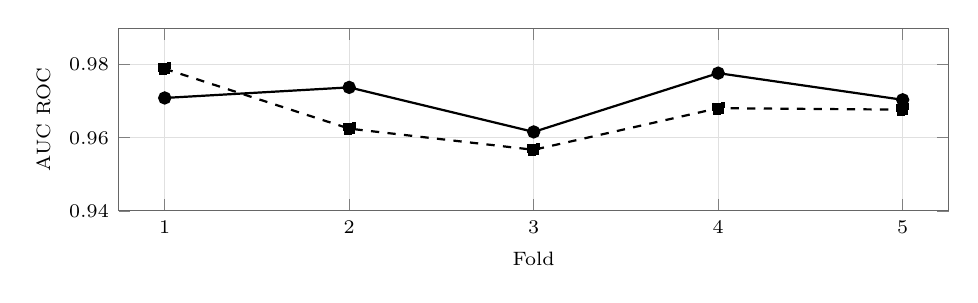
\begin{tikzpicture}
\begin{axis}[
  width=\linewidth,
  height=3.9cm,
  ymin=0.94,
  ymax=0.99,
  xmin=0.75,
  xmax=5.25,
  xtick={1,2,3,4,5},
  xlabel={Fold},
  ylabel={AUC ROC},
  grid=major,
  major grid style={black!12},
  axis line style={black!60},
  tick label style={font=\scriptsize},
  label style={font=\scriptsize}
]
\addplot[black,mark=*,thick] coordinates {
  (1,0.9709) (2,0.9738) (3,0.9616) (4,0.9777) (5,0.9704)
};
\addplot[black,mark=square*,thick,dashed] coordinates {
  (1,0.9789) (2,0.9625) (3,0.9567) (4,0.9681) (5,0.9677)
};
\end{axis}
\end{tikzpicture}
\end{minipage}
\hfill
\begin{minipage}{.49\textwidth}
\centering
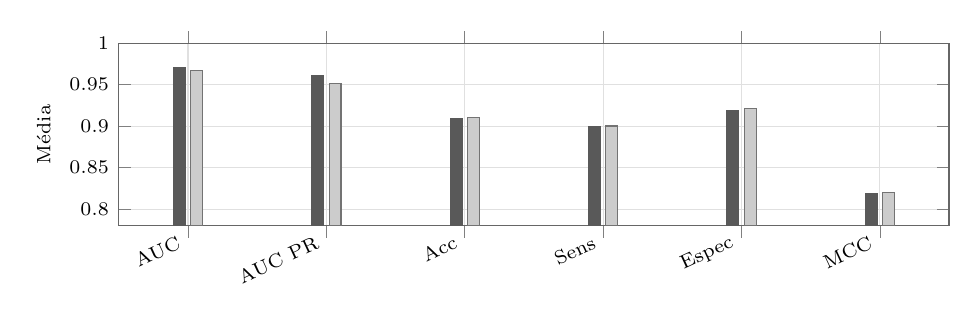
\begin{tikzpicture}
\begin{axis}[
  width=\linewidth,
  height=3.9cm,
  ybar,
  bar width=4.3pt,
  ymin=0.78,
  ymax=1.0,
  symbolic x coords={AUC,AUC PR,Acc,Sens,Espec,MCC},
  xtick=data,
  x tick label style={font=\scriptsize,rotate=25,anchor=east},
  ylabel={Média},
  tick label style={font=\scriptsize},
  label style={font=\scriptsize},
  grid=major,
  major grid style={black!12},
  axis line style={black!60}
]
\addplot[fill=black!65,draw=black!65] coordinates {
  (AUC,0.9709) (AUC PR,0.9607) (Acc,0.9091)
  (Sens,0.8994) (Espec,0.9188) (MCC,0.8189)
};
\addplot[fill=black!20,draw=black!55] coordinates {
  (AUC,0.9668) (AUC PR,0.9513) (Acc,0.9105)
  (Sens,0.9001) (Espec,0.9210) (MCC,0.8205)
};
\end{axis}
\end{tikzpicture}
\end{minipage}
\vspace{1mm}

{\scriptsize
\begin{tikzpicture}[baseline=-0.5ex]
\draw[black,thick] (0,0) -- (0.32,0);
\fill[black] (0.16,0) circle (1.2pt);
\end{tikzpicture}
ConvNeXt-Tiny\quad
\begin{tikzpicture}[baseline=-0.5ex]
\draw[black,thick,dashed] (0,0) -- (0.32,0);
\filldraw[black,fill=white] (0.16,0) rectangle +(2.2pt,2.2pt);
\end{tikzpicture}
ResNet-50\quad
\tikz{\filldraw[fill=black!65,draw=black!65] (0,0) rectangle (0.16,0.08);}
ConvNeXt-Tiny (barras)\quad
\tikz{\filldraw[fill=black!20,draw=black!55] (0,0) rectangle (0.16,0.08);}
ResNet-50 (barras)}
\caption{Comparação complementar com ResNet-50. À esquerda, AUC ROC por fold.
À direita, médias de métricas selecionadas na validação cruzada.}
\label{fig:comparacao-modelos}
\end{figure}

A Figura~\ref{fig:comparacao-modelos} evidencia que a diferença entre as
arquiteturas não é uniforme. A ResNet-50 superou a ConvNeXt-Tiny em AUC ROC
apenas no fold 1 ($+0{,}0080$), enquanto a ConvNeXt-Tiny ficou acima nos folds
2, 3, 4 e 5. Em acurácia balanceada, a ResNet-50 foi superior nos folds 1, 2 e
3, enquanto a ConvNeXt-Tiny foi superior nos folds 4 e 5. O maior ganho
operacional da ResNet-50 ocorreu no fold 1, com aumento de sensibilidade de
$+0{,}1032$; a maior perda ocorreu no fold 2, com redução de $-0{,}0419$ na
sensibilidade, compensada por aumento de especificidade de $+0{,}0567$.

\begin{figure}[H]
\centering

\includegraphics[width=.82\textwidth]{predicoes_convnext_cv_sem_borda.png}
\caption{Exemplos qualitativos de predições da ConvNeXt-Tiny. As probabilidades
correspondem à classe anormal; valores próximos de 0 indicam maior confiança em
normalidade e valores próximos de 1 indicam maior confiança em anormalidade. A
figura é ilustrativa e não substitui as métricas calculadas nos folds.}
\label{fig:predicoes}
\end{figure}

A Figura~\ref{fig:predicoes} complementa a análise quantitativa com predições
corretas e erros próximos ao limiar. Os falsos positivos tendem a probabilidades
intermediárias ou moderadamente altas, coerentes com estruturas nucleares
salientes em alguns recortes; os falsos negativos concentram-se em amostras
anormais com probabilidade próxima de 0,50 ou menor, quando a evidência
morfológica do recorte isolado é insuficiente. Em conjunto, a ConvNeXt-Tiny
apresenta desempenho médio elevado, mas a triagem automática deve ser
interpretada como ferramenta de priorização e apoio, não como substituto direto
da avaliação citopatológica.
